\section*{Chương 2: Thuật toán và chương trình trên Matlab}
\addcontentsline{toc}{section}{Chương 2: Giải thuật nén ảnh và code Matlab}

\subsection*{1. Thuật toán nén ảnh}
Trong thực tế khi thực hiện phép nhân ma trận $B = HAH^T$ độ phức tạp thuật toán tăng lên mức 
$O(N^3)$ gây sự lãng phí tài nguyên và thời gian tính toán. Một cách tiếp cận với phép biến đổi Haar
chính là dùng thuật toán \textit{Fast Haar Wavelet Transform (FWT)} giúp giảm độ phức tạp
thuật toán xuống còn \textit{O(N)}. 

Về mặt lý thuyết ta có thể liên tục băm nhỏ một bức ảnh đến khi thành phần $LL$ chỉ còn 1 pixel duy nhất.
Ví dụ một bức ảnh độ phân giải $512 \times 512$ pixels sau 3 lần biến đổi còn lại $64 \times 64$ pixels.
Lúc này bản thân bức ảnh đã rất nhỏ, cùng với việc cắt ngưỡng quá mức có thể xóa mất những chi tiết quan trọng
khiến việc khôi phục ảnh gốc mất mát nhiều dữ liệu hơn dự tính. Do đó chúng ta có thể lựa chọn
số lần phân nhỏ ảnh gốc để đồng thời kiểm soát chất lượng bức ảnh và vẫn giữ được sự tối ưu dữ liệu.

Do đã biết bản chất phép biến đổi Haar là lấy trung bình và sai khác ta có thể giải thích thuật toán như sau:
\begin{enumerate}
    \item Khởi tạo một cell detail để lưu các ma trận chi tiết đã được phân tách.
    \item Cho vòng lặp chạy từ level 1 đến level đã chọn.
    \item Tạo các ma trận $LL$, $HL$, $LH$, $HH$ bằng một phần tư ảnh gốc.
    \item Trích xuất tập hợp $A, B, C, D$ lần lượt là ma trận các pixel ở góc trái trên cùng, góc phải trên cùng, góc trái dưới cùng, góc phải dưới cùng của mỗi khối vuông 4 pixel.
    \item Tính toán các ma trận $LL, HL, LH, HH$ theo công thức và lưu vào detail tại từng level.
    \item Gán ảnh gốc là ma trận $LL$ sau đó thực hiện tiếp biến đổi nếu chưa đi hết level đã chọn.
\end{enumerate}

Dưới đây là hàm phân giải ảnh theo thuật toán:

\begin{lstlisting}[language=Matlab]
function [LL, detailArr] = haar_decompose(img, level)
    LL = double(img);
    detailArr = cell(level, 3); 
    
    for i = 1:level
        [rows, cols] = size(LL);
        
        LL = LL(1:2*floor(rows/2), 1:2*floor(cols/2));
        
        A = LL(1:2:end, 1:2:end);
        B = LL(1:2:end, 2:2:end);
        C = LL(2:2:end, 1:2:end);
        D = LL(2:2:end, 2:2:end);
        
        LLNew = (A + B + C + D) / 2;
        HL = (A + B - C - D) / 2;
        LH = (A - B + C - D) / 2;
        HH = (A - B - C + D) / 2;

        detailArr{i, 1} = HL;
        detailArr{i, 2} = LH;
        detailArr{i, 3} = HH;
        s
        LL = LLNew; 
    end
end
\end{lstlisting}

\subsection*{2. Thuật toán cắt ngưỡng}

Giải thích thuật toán cắt ngưỡng:
\begin{enumerate}
    \item Cho một vòng lặp qua từng level, đối với từng level duyệt qua các ma trận chi tiết $HL, LH, HH$.
    \item Trong từng ma trận chi tiết thực hiện ép ngưỡng các phần tử dó giá trị tuyệt đối nhỏ hơn ngưỡng.
    \item Lưu lại ma trận chi tiết đã chỉnh sửa.
\end{enumerate}

Dưới đây là code thực hiện thuật toán trên:
\begin{lstlisting}[language=Matlab]
    for i = 1:level
        for j = 1:3
            coEff = app.detailArrAfter{i, j};
            coEff(abs(coEff) < tau) = 0;
            app.detailArrAfter{i, j} = coEff;
        end
    end

\end{lstlisting}


\subsection*{3. Thuật toán giải nén}

Giải thích thuật toán giải nén:
\begin{enumerate}
    \item Cho vòng lặp chạy từ level cao nhất trở về level thấp nhất.
    \item Tạo ma trận ảnh trống kích thước gấp đôi ma trận ảnh $LL$.
    \item Đối với mỗi level lấy thành phần $LL$ làm ảnh gốc để tái tạo các ảnh khác.
    \item Tạo ma trận $A, B, C, D$ và tính toán.
    \item Đưa từng phần tử của các ma trận $A, B, C, D$ vào các vị trí tương ứng mới.
\end{enumerate}

Dưới đây là code thực hiện thuật toán trên:
\begin{lstlisting}[language=Matlab]
    function img_recon = haar_reconstruct(LL, Details, level)
        img_recon = LL;
        for i = level:-1:1
            HL = Details{i, 1};
            LH = Details{i, 2};
            HH = Details{i, 3};

            [m, n] = size(img_recon);
            temp = zeros(2*m, 2*n);

            A = (img_recon + HL + LH + HH) / 2;
            B = (img_recon + HL - LH - HH) / 2;
            C = (img_recon - HL + LH - HH) / 2;
            D = (img_recon - HL - LH + HH) / 2;

            temp(1:2:end, 1:2:end) = A;
            temp(1:2:end, 2:2:end) = B;
            temp(2:2:end, 1:2:end) = C;
            temp(2:2:end, 2:2:end) = D;

            img_recon = temp;
        end
    end
\end{lstlisting}

\subsection*{4. Chương trình trên Matlab}

\begin{figure}[H]
    \centering
    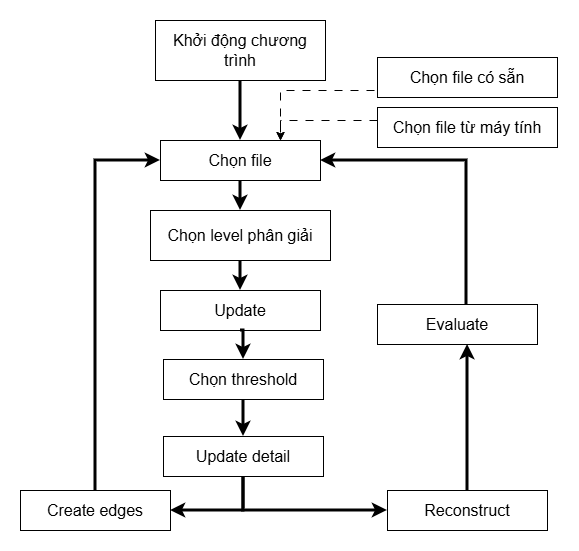
\includegraphics[width=1\textwidth]{AppFlowchart.png}
    \caption{Lưu đồ chương trình trên Matlab.}
\end{figure}

Cấu trúc chương trình có thể được diễn giải thành các bước sử dụng như sau:
\begin{enumerate}
    \item Khởi động chương trình bằng phần mềm Matlab. Chương trình được khởi động sẽ hiển thị giao diện người dùng.
    \item Nhấn chọn hình ảnh đã có sẵn hoặc nhấn \textit{Browse} để chọn ảnh bất kì trong máy tính.
    \item Sau khi chọn ảnh, hình ảnh sẽ được hiển thị. Mục \textit{Level} cũng sẽ được update để người dùng chọn cấp độ phân giải.
    \item Sau khi chọn độ phân giải người dùng nhấn \textit{Update} để tiến hành biến đổi ảnh thành các thành phần xấp xỉ và sai khác.
    \item Người dùng sau đó có thể chọn \textit{Threshold = 0} để thực hiện nén không mất dữ liệu hoặc \textit{Threshold $>$ 0} để thực hiện nén mất dữ liệu và nhấn \textit{Update detail} để cắt ngưỡng.
    \item Tiếp theo người dùng có thể chọn chức năng chính là \textit{Reconstruct} để khôi phục ảnh và nhấn \textit{Evaluate} để đánh giá mức độ khôi phục. Hoặc người dùng có thể nhấn \textit{Create edges} để thực hiện tính năng phụ là phân tích cạnh của vật thể trong ảnh.
    \item Người dùng có thể tiếp tục đánh giá phân tích ảnh bằng cách lặp lại quy trình trên.
\end{enumerate}

\noindent \textbf{Giao diện chương trình:}
\begin{figure}[H]
    \centering
    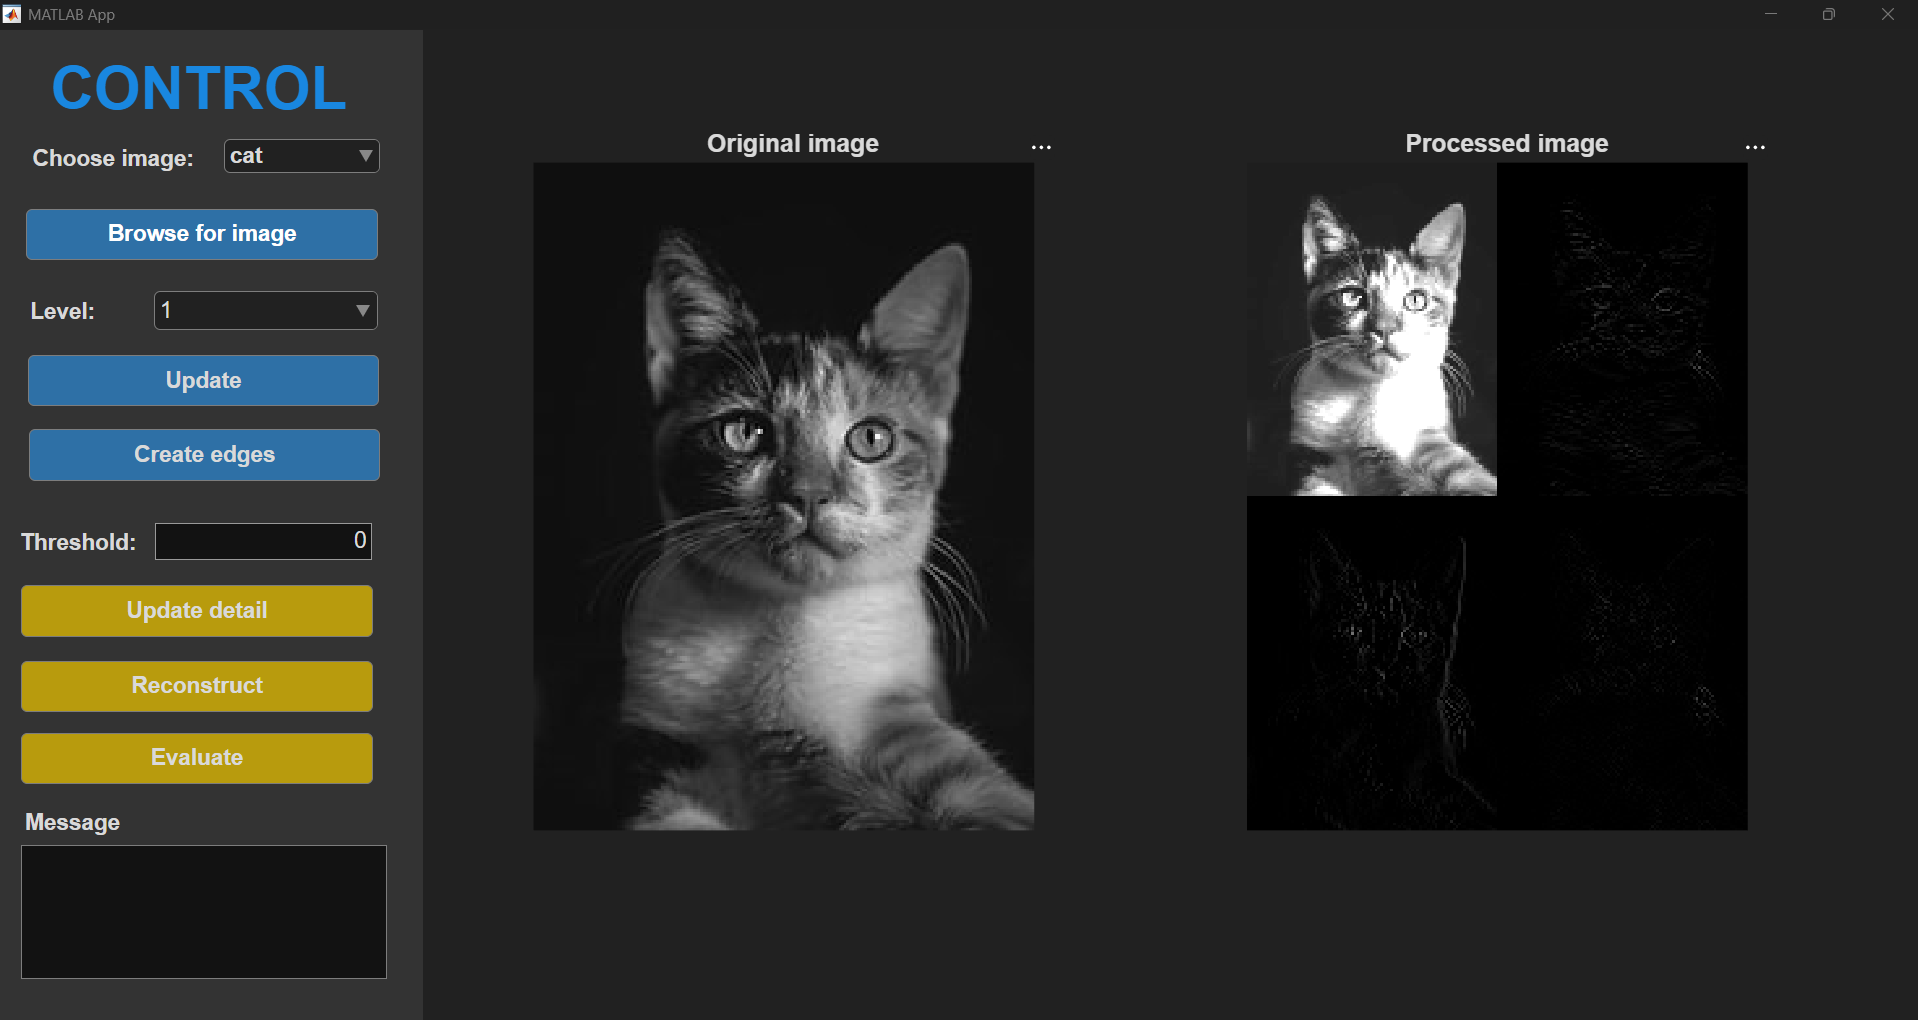
\includegraphics[width=1\textwidth]{App_UI.png}
    \caption{Giao diện chương trình trên Matlab.}
\end{figure}
